\label{sec:detector-mu}
Outside the calorimeters sits the muon spectrometer show in Fig.\ref{fig:detector-mu}. Even though the muon spectrometer only serves to measure and detect the muons, it has profound importance for physics. One of the early concerns for ATLAS and CMS experiments are that the detector's capability to handle the high rate of LHC collisions. The ID and calorimeters could potentially be blacked out. One channel that would still allow us to study the Higgs in such circumstance is the Higgs to four muons, the background of which is also low rate. Hence the muon system was the safety insurance for ATLAS to produce meaningful physics result historically. The entire muon spectrometer is divided into four parts\cite{ATLASDetector}. The Monitored Drift Tubes (MDT) and Cathode Strip Chambers (CSC) are the precision chambers used for precision muon measurements, while the Resistive Plate Chambers (RPC) and Thin Gap Chambers (TGC) are used for fast muon triggering. Muons entered into the muon spectrometer are bent the second time by the 4T toroid magnetic field. 

\begin{figure}[htpb!]
\begin{center}
  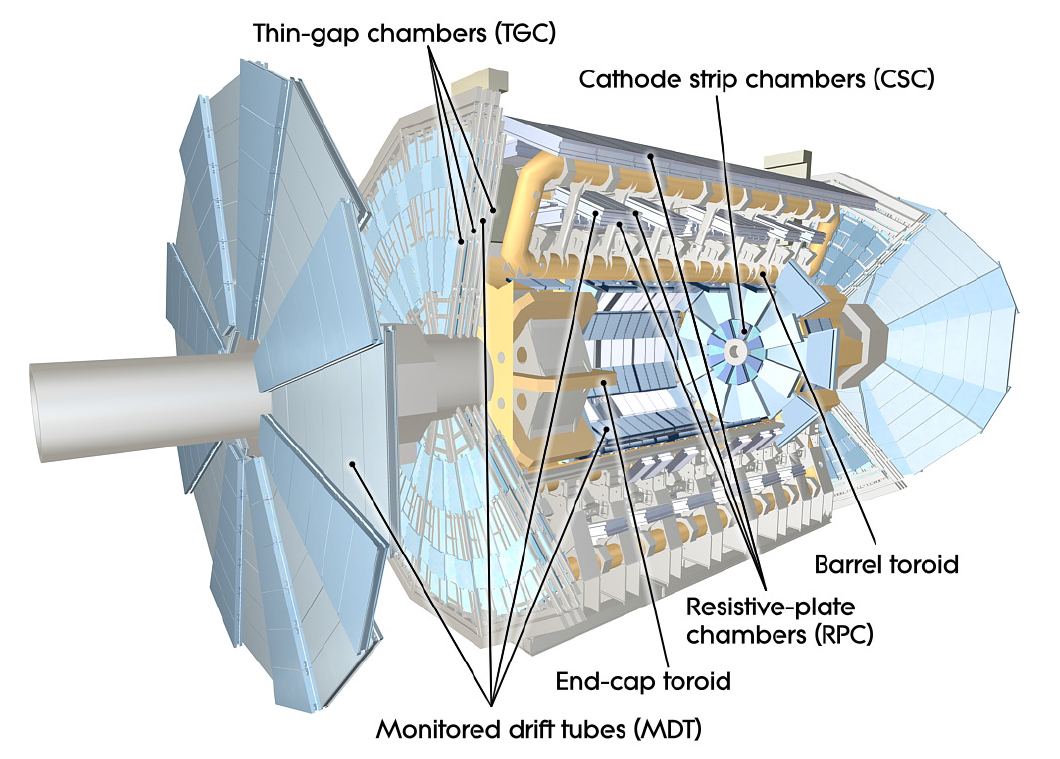
\includegraphics[width=0.8\linewidth]{figures/detector/muon}
\caption{View of ATLAS muon spectrometer}
\label{fig:detector-mu}
\end{center}
\end{figure}


There are three layers of precision chambers at the barrel of the detector and four layers at the endcaps located at the ATLAS large wheels. Most of the layers are MDT which cover $|\eta|<2.7$ except for the innermost layer of the endcap, which uses CSC due to very high rate forward rate. The MDT consists of 29.97mm pressurized drift tubes filled with $Ar$ and $CO_2$ gas and provide $35\mu m$ resolution in $z$. Within the CSC active gas (also $Ar$ and $CO_2$) volume there are perpendicular cathode strips such that CSC can provide a two dimensional coordinate system. The CSC safe operating count rate is 1000 $Hz/cm^2$ much higher than the 150 $Hz/cm^2$ of the MDT with comparable resolution. The RPC modules are made of two resistive plates and apply 4.9$kV/mm$ to the gas mixture filled in the short 2$mm$ space in between ($C_2H_2F_4/Iso-C_4H_{10}/SF_6$). They are inserted near the MDT and with reasonable cost can read out safely at 1000 $Hz/cm^2$. The TGC essentially has the same design as the CSC but with smaller wire and cathode spacing to allow faster electron drifts. 

